\part{Évaluation des outils et méthodes : bilan et perspectives}
\chapter{Performance des applications}
    \section{\cvt}   
    En examinant le graphique des tailles des fichiers PNG avant et après conversion avec GIMP et \py, il est clair que les fichiers PNG originaux sont généralement beaucoup plus volumineux que leurs versions converties en JPEG. Par exemple, le fichier \texttt{3DM\_FN170\_Mallet\_0.5mm\_filled\_ZG}, dont la taille originale est de 69,3 Mo, est compressé à 285,4 Ko avec GIMP et à 145,2 Ko avec \py. Cette réduction significative des tailles des fichiers PNG en JPEG est évidente pour tous les modèles étudiés. 
    
    Les différences entre les tailles obtenues avec GIMP et \py montrent que \py atteint des tailles de fichiers légèrement plus petites dans certains cas, ce qui pourrait refléter une compression plus efficace. Par exemple, pour le modèle \texttt{3DM\_TT95\_BL4\_1mm\_ZG}, \py réduit la taille à 294 Ko, contre 490,6 Ko avec GIMP. Cette tendance indique que l'application \py \cvt pourrait offrir une meilleure compression pour les fichiers JPEG, ce qui est important pour optimiser le stockage et la gestion des fichiers.

        \begin{table}[htbp]
            \centering
            \resizebox{\textwidth}{!}{
                \begin{tabular}{|l|l|l|l|}
                \hline
                \rowcolor{gray!20} % première ligne grise
                \textbf{Nom du fichier PNG} & \textbf{Taille originale} & \textbf{GIMP (JPEG)} & \textbf{Python (JPEG)} \\ \hline
                3DM\_FN170\_Mallet\_0.5mm\_filled\_ZG & 69,3 Mo  & 285,4 Ko  & 145,2 Ko \\ \hline
                3DM\_TT95\_BL4\_1mm\_ZG               & 38,9 Mo  & 490,6 Ko  & 294 Ko   \\ \hline
                3DM\_FN312\_FN313\_FN749\_FN789\_Sandstone\_0.5mm\_filled\_ZG & 116,9 Mo & 411,6 Ko & 217,8 Ko \\ \hline
                3DM\_FN571\_Sandstone\_0.5mm\_filled\_ZG & 42,9 Mo  & 244,8 Ko  & 134,1 Ko \\ \hline
                3DM\_TT95\_BL3\_1mm\_ZG               & 25,1 Mo  & 562,7 Ko  & 383,6 Ko \\ \hline
                \end{tabular}}
                \caption{Comparaison des tailles de fichiers avant et après conversion (GIMP et \cvt)}
        \end{table}

        % Graphe \cvt
        \begin{figure}[h!]
            \centering
            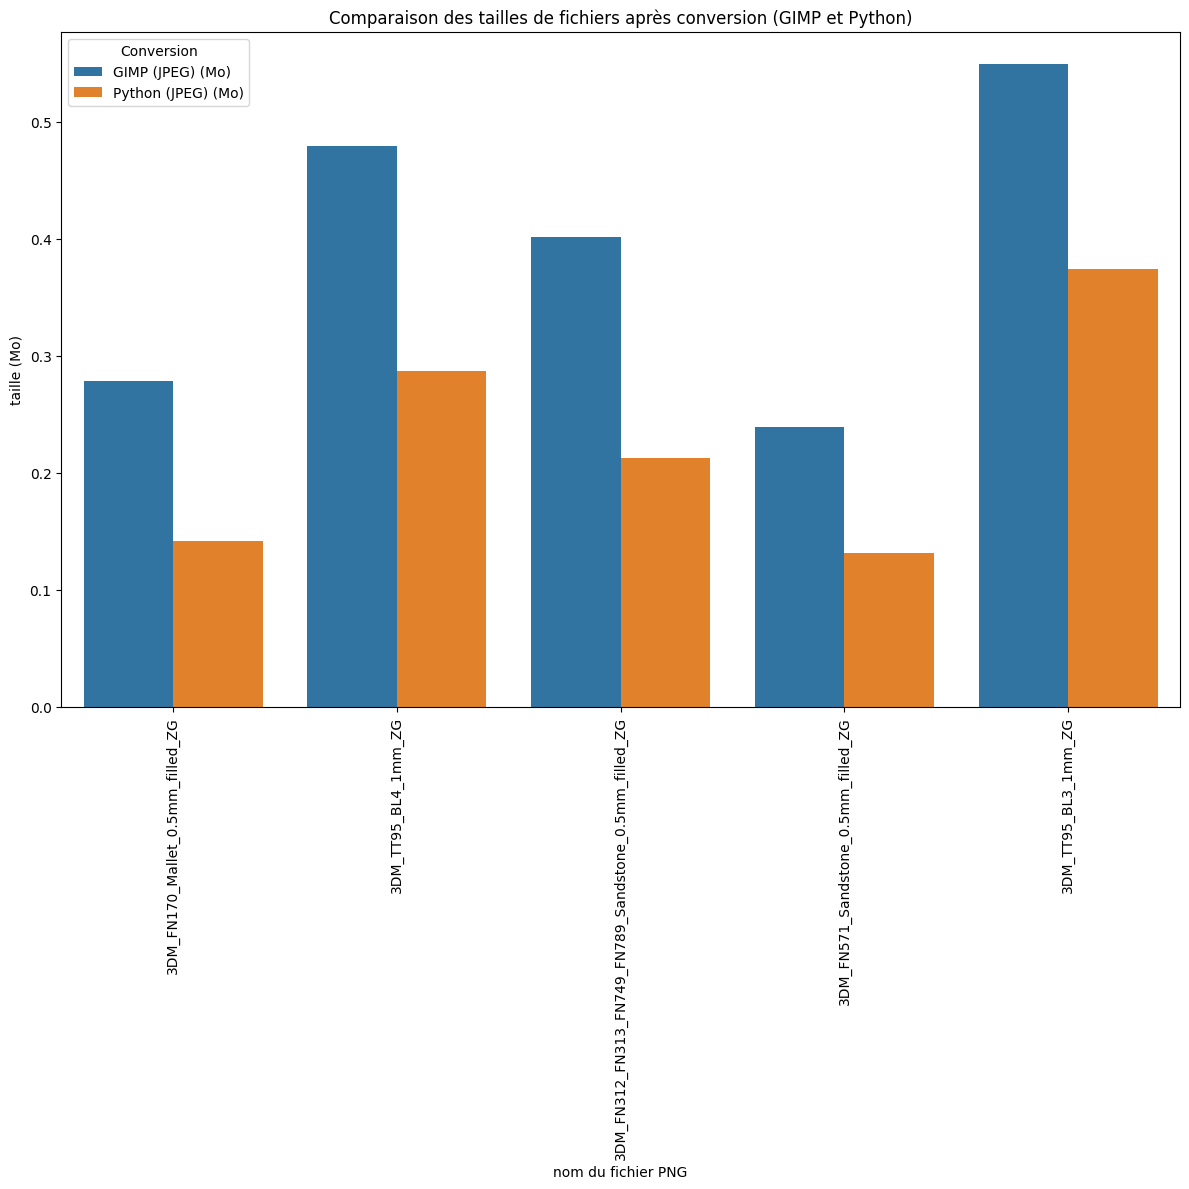
\includegraphics[width=13cm]{02_images/part_03/03_cvt_dv.png}
            \caption{Performance \cvt}
        \end{figure}
        
        
    \section{\msh}
 
    L'analyse des données sur les tailles des fichiers avant et après conversion révèle des informations cruciales sur l'efficacité des méthodes de compression utilisées. La réduction de la taille des fichiers est un facteur important dans le traitement et la gestion des données numériques, et les résultats obtenus permettent de comparer directement l'efficacité de différentes techniques de conversion.

    L'analyse du graphique illustrant les tailles des fichiers avant et après conversion avec MeshLab et \py met en évidence une réduction notable de la taille des fichiers grâce à l'utilisation de MeshLab. Par exemple, le fichier \texttt{3DM\_FN170\_Mallet\_0.5mm\_ZG}, initialement de 91 Mo, est réduit à seulement 6,78 Mo après conversion avec MeshLab, ce qui indique une compression significative. Cette tendance se confirme pour tous les modèles examinés, où MeshLab permet de réduire considérablement la taille des fichiers tout en limitant le nombre de sommets à 65 000. En comparaison, les conversions réalisées avec \py montrent une augmentation significative des tailles de fichiers dans la plupart des cas. Par exemple, le modèle \texttt{3DM\_TT95\_BL4\_1mm\_ZG} passe de 21,4 Mo avec MeshLab à 175,56 Mo avec Python, indiquant une augmentation notable de la taille des fichiers. 
    
        \begin{table}[htbp]
        \centering
        \resizebox{\textwidth}{!}{
            \begin{tabular}{|l|l|l|l|}
            \hline
            \rowcolor{gray!20} % première ligne grise 
            \textbf{Nom du modèle 3D} & \textbf{Taille originale} & \textbf{MeshLab (65k sommets)} & \textbf{Python (65k sommets)} \\ \hline
            3DM\_FN170\_Mallet\_0.5mm\_ZG & 91 Mo  & 6,78 Mo  & 21,56 Mo \\ \hline
            3DM\_TT95\_BL4\_1mm\_ZG      & 1,1 Go & 21,4 Mo  & 175,56 Mo \\ \hline
            3DM\_FN312\_FN313\_FN749\_FN789\_Sandstone\_0.5mm\_filled\_ZG & 625 Mo & 7,06 Mo  & 107,46 Mo \\ \hline
            3DM\_FN169\_Mallet\_ZG       & 157 Mo & 14,4 Mo  & 14,7 Mo \\ \hline
            3DM\_FN1848\_Mortar-3Cone\_Imprints & 22,8 Mo & 12,8 Mo & 4,6 Mo \\ \hline
            \end{tabular}}
        \caption{Comparaison des tailles de fichiers avant et après conversion avec MeshLab et \msh}
        \end{table}

        % Graphe \mshs
        \begin{figure}[h!]
            \centering
            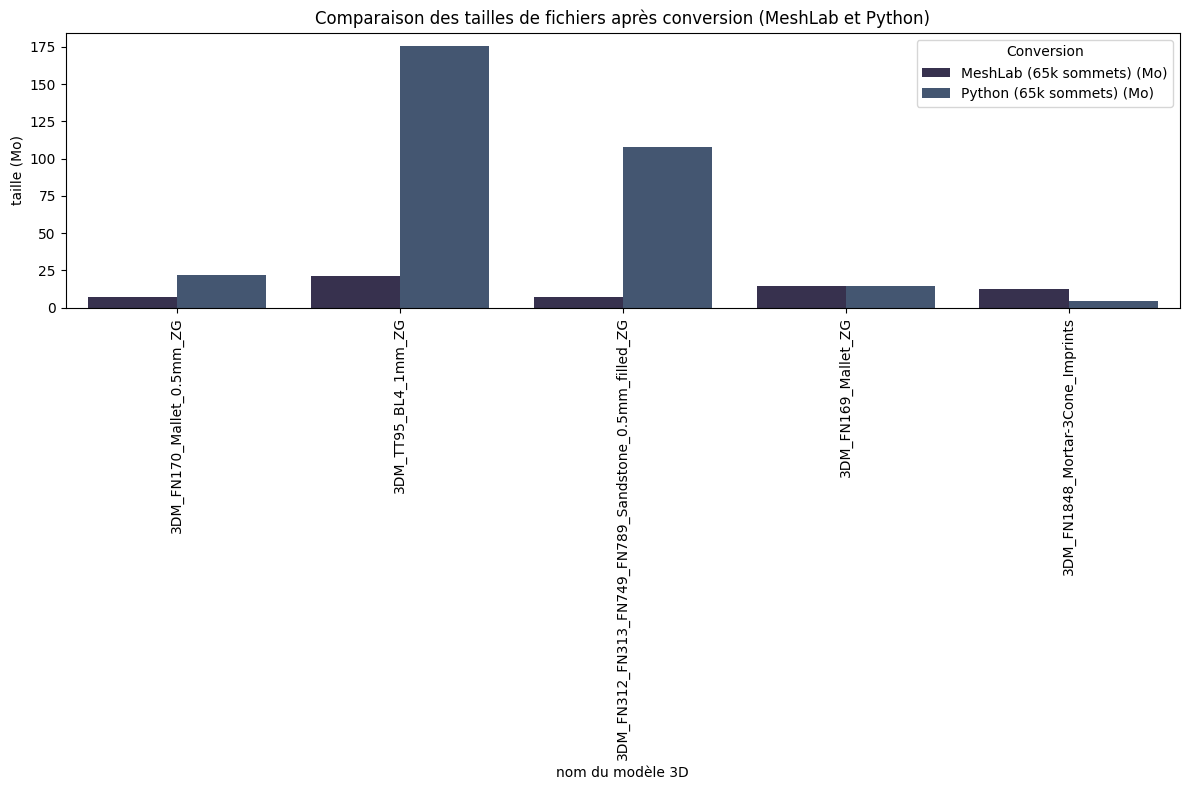
\includegraphics[width=13cm]{02_images/part_03/04_msh_dv.png}
            \caption{Performance \msh}
        \end{figure}

        Cela suggère que l'application \py \msh n'a pas encore été aussi efficace dans la gestion de la compression des fichiers pour les données 3D que MeshLab. Une explication plausible pour la baisse significative des performances pourrait résider dans l'utilisation de la bibliothèque Open3D. En effet, cette dernière n'offre pas les mêmes options de configuration que MeshLab. De plus, bien que la bibliothèque PyMeshLab offrait les mêmes options de configuration que MeshLab \footnote{Voir \cite{pymeshlab_decimation}.}, elle engendrait des boucles infinies lors de la conversion de fichiers volumineux. Pour de futures implémentations, il pourrait être envisagé d'utiliser Open3D ou d'explorer d'autres solutions au sein de PyMeshLab.
        
        
\chapter{Perspectives d'évolution : fonctionnalités supplémentaires}
    \section{Implémentations plus imminentes}

    Le développement logiciel est un processus collaboratif. Un programme est rarement le fruit du travail d'un seul développeur, mais plutôt le résultat d'une chaîne de contributions successives. Les codes sources sont partagés, modifiés, améliorés par différents acteurs au fil du temps. Cette nature collaborative du développement nécessite également une gestion rigoureuse des versions et une documentation précise pour garantir la cohérence du projet. Pour cette étude, les applications ont encore des implémentations à faire et voire des améliorations conséquentes.
    
    En ce qui concerne la gestion d'erreur, les deux applications \cvt et \msh en présentent une gestion sommaire. Seules les erreurs 404 et 500 ont été traitées, respectivement avec un modèle de \eng{template} qui affiche des images lors de l'erreur. Il serait intéressant de travailler ces erreurs pour les prochaines étapes du développement.

    Il serait pertinent d'intégrer des écrans de chargement lors du traitement de fichiers volumineux. L'objectif est de maintenir l'utilisateur au sein de l'application pendant toute la durée de l'opération. Une simple barre de progression, dont de noMoreux modèles sont disponibles sur Bootstrap par exemple, pourrait suffire \footnote{ces icônes de chargement d'un composant ou d'une page sont appelés de \eng{spinners}. Pour les exemples, Voir \cite{bootstrapspinners}.}.
    
    \section{D'autres implémentations possibles}
    \cvt et \msh, comme dit, ont été codés en \py à cause des raisons spécifiés dans la chapitre 4, à savoir : . néanmoins, ces applications peuvent, une fois finies et distribuées sur le \eng{DockerHub} de \dsc, être codées avec d'autres langages dont l'accent est mis sur la gestion de données et la performance, à l'instar de \textsc{rust} et \textsc{go}. 

    Les temps de réponse, en particulier pour les fonctionnalités qui nécessitent le traitement de grandes quantités de données, serait aussi une possibilité d'amélioration. Cela pourrait inclure la refactorisation du code pour le rendre plus efficace, l'implémentation de techniques de mise en cache, qui n'ont pas pu être développés lors du stage. 
    
    Par ailleurs, le recours à l'apprentissage automatique offre de nouvelles perspectives pour optimiser le processus de \msh. En entraînant un modèle sur un ensemble de données variées, il devient possible d'automatiser la classification des images et des objets, et ainsi de proposer des traitements adaptés à chaque type de fichier. Par exemple, en fonction de la présence ou de l'absence de textures, le modèle pourrait sélectionner automatiquement les algorithmes de conversion les plus pertinents (par exemple, un méthode A pour les fichiers sans texture et un méthode B pour les fichiers texturés). Cette approche permettrait de personnaliser davantage le processus de conversion et d'améliorer la qualité des résultats.

    L'interface utilisateur de l'application pourrait également être enrichie afin de faciliter l'utilisation et d'améliorer l'expérience utilisateur. En effet, il serait pertinent de développer des fonctionnalités permettant d'identifier rapidement les fichiers téléchargés.

    Pour répondre aux besoins des utilisateurs ayant de grands volumes de fichiers à convertir, il serait intéressant d'implémenter une fonctionnalité permettant de traiter plusieurs fichiers simultanément. Cette option permettrait de gagner en productivité et de simplifier le flux de travail. En outre, la création d'une liste de téléchargement pourrait être proposée afin de permettre à l'utilisateur de suivre l'avancement des conversions et de télécharger les fichiers résultants de manière organisée.
    
    En ce qui concerne \diiif, même si l'application n'est pas finalisée, il est concevable de tirer quelques pistes : dans un premier temps, l'inspiration serait créer une application intuitive, similaire à \cvt et \msh, car en termes d'\ux, elles sont intéressantes pour avoir intégré des éléments importants du \gco ; deuxièmement, transformer le code en application et le diffuser sur \textsc{docker} serait aussi un moyen de le rendre accessible au plus grand noMore d'utilisateurs possible.

\chapter{Outils de travail}
    \section{Aspects techniques}
    Tout d'abord, l'étude a bénéficié d'un MacBook Air équipé d'un processeur M1 d'Apple Silicon, offrant ainsi un outil performant et portable pour mener à bien les différentes tâches de la recherche.
    
    De plus, un disque dur externe contenant l'ensemble des données du projet DaSCH a été mis à disposition, permettant ainsi la mise en œuvre de \eng{pipelines} d'analyse automatisés. La portabilité de ce support a favorisé une grande flexibilité dans le déroulement des travaux.

    En somme, l'ordinateur ainsi que la disponibilité des données ont permis de mener des analyses approfondies, notamment des tests de performance, favorisant ainsi une exploitation optimale des données. Le télétravail a également été facilité grâce à cette configuration. À l'issue du stage, le MacBook Air a été restitué. En revanche, le disque dur externe nous a été attribué.

    \section{Gestion du temps}    
    Le déroulement du stage s’est distingué par une grande autonomie et une organisation méthodique, structurée en petites tâches hebdomadaires, gérées à l’aide de l’outil \textsc{trello}. Ce tableau de tâches, partagé avec \rg, la superviseure du stage, a permis un suivi rigoureux de l’avancement des \eng{pipelines} tout en servant de base pour les réunions hebdomadaires. Ces réunions, associées à cette approche structurée, ont favorisé une productivité réaliste, offrant un équilibre entre suivi et liberté. Elles ont également permis l’établissement d’un dialogue constructif, où des solutions, réflexions, et pistes d’amélioration ont pu être explorées pour débloquer certains problèmes, tout en offrant une compréhension approfondie du métier de la superviseure.

        % structure GitHub du \cvt
        \begin{figure}[h!]
            \centering
            
\includegraphics[width=10cm]{02_images/part_03/01_trello_logo.png}
            \caption{Logo de l'application \textsc{trello}}
        \end{figure}
    
    Au sein du projet DaSCH, la communication se faisait principalement par le biais d'une suite d'outils \eng{Google Workspace}, mettant à disposition des chercheurs une boîte mail professionnelle et un espace de travail collaboratif. Les échanges instantanés, particulièrement fréquents, étaient privilégiés via la messagerie instantanée de \eng{Google Chat}. Par ailleurs, l'outil \eng{Google Meet} était largement utilisé pour les réunions en ligne, offrant ainsi la possibilité de conférences et de partages d'écran en temps réel.

    En ce qui concerne les réunions, deux formats principaux étaient privilégiés. Des réunions d'équipe hebdomadaires permettaient de faire le point sur l'avancement du projet et de coordonner les tâches. Afin d'assurer un suivi régulier de l'exécution des codes, comme mentionné, il y avait aussi des réunions hebdomadaires dédiées. Ces rendez-vous réguliers ont permis de garantir une progression efficace du développement et de lever rapidement les éventuelles difficultés rencontrées. Cela n'a pas empêché de réaliser d'autres réunions entre les meMores de l'équipe, mais celles-là étaient moins régulières. 
    
    En ce qui concerne le travail de codage, un accord a été établi dès le début du stage pour que les horaires du stage soient organisées selon la technique Pomodoro, qui est une technique créée en 1992 pour réaliser une gestion efficace du temps \footnote{D'après Cirillo, cette technique, répandu dans le milieu du mangament depuis le final des années 90, a pour but, entre autres, améliorer le processus de travail et d'études. Voir \cite[p.~20]{cirillo2009}.}. Pour ce faire, l’application utilisée pour compter les minutes, nommée \textsc{flow}, a permis de structurer le temps en quatre sessions de 25 minutes avec des pauses de 5 minutes, suivies d’une longue pause de 30 minutes après le quatrième cycle. Cette méthode visait à améliorer la concentration lors de l’exécution des tâches, rendant le travail plus efficace. Dans le cadre de ce stage, la technique a contribué au développement de deux applications tout en aidant à trouver un rythme de travail adéquat.

        % structure GitHub du \cvt
        \begin{figure}[h!]
            \centering
            
\includegraphics[width=10cm]{02_images/part_03/02_flow_macos_logo.png}
            \caption{Logo de l'application \textsc{flow}, disponible que pour les \eng{macOS} et \eng{iOS}}
        \end{figure}

    La participation aux réunions, bien que non obligatoire pour les stagiaires, s'est révélée extrêmement bénéfique. Ces réunions ont offert une compréhension globale du travail, ainsi qu'une vision claire du fonctionnement quotidien d'un groupe de travail en sciences humaines. Cette immersion a permis la conception d'applications réalistes, tenant compte des spécificités de chaque groupe, et l'identification d'axes d'amélioration. De plus, cette expérience a enrichi la maîtrise de l'anglais et a fourni l'opportunité d'apprendre à gérer un projet de codage en collaboration avec plusieurs acteurs, facilitant ainsi une meilleure compréhension de la contribution de chaque partie à la réussite du projet.

    En conclusion, ce stage a été une expérience enrichissante à plusieurs niveaux. L’autonomie dans l’organisation du travail, la méthode structurée de gestion du temps, et l’implication active dans les réunions ont non seulement permis la réalisation d’applications concrètes mais ont aussi favorisé un apprentissage profond du fonctionnement d’un projet de données en sciences humaines. Ces compétences acquises, tant techniques que relationnelles, constituent une base solide pour mes futurs projets professionnels.